% This part is to be filled by Johann
\subsection{Christofides Algorithm}

\begin{frame}[t]{Christofides Algorithm}
  \begin{itemize}
    \item Assumption: the input graph is metric, i.e. the triangle inequality holds
    \pause
    \item the algorithm goes as following \cite{christofides_worst-case_1976}:
      \begin{enumerate}
        \item calculate the MST
        \pause
        \item calculate a matching in the complete graph of minimum weight, over all vertices, that have odd degree in the MST
          \begin{itemize}
            \item see also next slides
          \pause
            \item parallelization: mostly in this step
          \end{itemize}
        \pause
        \item combine the MST and the matching into one multigraph
        \pause
        \item find an eulerian cycle through the multigraph
        \pause
        \item make the eulerian cycle hamiltonian
      \end{enumerate}
  \end{itemize}
\end{frame}

\begin{frame}[t]{Christofides Algorithm: Where To Find A Matching?}
  Complete input graph with highlighted MST:

  \begin{tikzpicture}
    \graph { subgraph K_n [n=5, clockwise, edges=gray];
      (1) --[thick] (2);
      (1) --[thick] (5);
      (5) --[thick] (4);
      (1) --[thick] (3); };
    
  \end{tikzpicture}

  Vertices with odd degree: $1,2,3,4$. $\hookrightarrow$ Find a matching over these vertices (blue):

  \begin{tikzpicture}
    \graph { subgraph K_n [n=5, clockwise, edges=gray];
      (1) --[thick] (2);
      (1) --[thick] (5);
      (5) --[thick] (4);
      (1) --[thick] (3);
      (4) --[thick, blue] (3);
      (1) --[thick, blue, bend left] (2);
    };
  \end{tikzpicture}

  Note: edge weights are left out for simplicity
\end{frame}

\begin{frame}[t]{Christofides Algorithm: Finding A Matching}
  Finding a minimum cost matching:
  \begin{itemize}
    \item exact solution:
      \begin{itemize}
        \item uses a sophisticated algorithm (the \href{https://en.wikipedia.org/wiki/Blossom_algorithm}{blossom algorithm})
        \item hard to parallelize
        \item slow (uses a lot of HashSets)
      \end{itemize}
      \pause
    \item randomized approximate solution:
      \begin{itemize}
        \item idea: guess a matching and do some randomized improvements.\\Repeat this and take the best matching
        \item easy to implement
        \item easy to parallelize
      \end{itemize}
  \end{itemize}
\end{frame}

\begin{frame}[t]{Christofides Algorithm: Randomly Finding A Matching}
  \vfill
  Finding a matching: the graph is complete \& has even amount of vertices (trivial)

  \begin{enumerate}
    \item Given the list of all vertices $[0,1,2,3,4,5,6,7]$
    \item randomly scramble the list: $[2,1,0,3,7,5,6,4]$
    \item interpret the list as a matching: $[[2,1],[0,3],[7,5],[6,4]]$
  \end{enumerate}
  \vfill
\end{frame}

\begin{frame}[t]{Christofides Algorithm: Improving A Matching Of 4 Vertices}
  \vfill
  Improving a matching on 4 vertices: easy: only 3 cases to consider:
  \vfill

  \hfill
  \begin{tikzpicture}
    \node (1) at (0,1) {1};
    \node (2) at (0,0) {2};
    \node (3) at (1,1) {3};
    \node (4) at (1,0) {4};
    \graph { (1) -- (2); (3) -- (4)  };
  \end{tikzpicture}, \hfill or \hfill
  \begin{tikzpicture}
    \node (1) at (0,1) {1};
    \node (2) at (0,0) {2};
    \node (3) at (1,1) {3};
    \node (4) at (1,0) {4};
    \graph { (1) -- (3); (2) -- (4)  };
  \end{tikzpicture} \hfill or \hfill
  \begin{tikzpicture}
    \node (1) at (0,1) {1};
    \node (2) at (0,0) {2};
    \node (3) at (1,1) {3};
    \node (4) at (1,0) {4};
    \graph { (1) -- (4); (2) -- (3)  };
  \end{tikzpicture}

  \vfill
  Chose the matching with the lowest cost.
  \vfill
\end{frame}

\begin{frame}[t]{Christofides Algorithm: Randomly Improving A Matching}
  \vfill
  Improving a matching:\\
  improve pairs of edges:
  \begin{enumerate}
    \item Given a matching $[[2,1],[0,3],[7,5],[6,4]]$
    \item randomly scramble the list: $[[7,5],[0,3],[2,1],[6,4]]$ \label{itemize:random_edge_scramble}
    \item consider consecutive blocks of two edges: $[7,5],[0,3]$ and $[2,1],[6,4]$
    \item for a block of two edges, consider the other two possible matchings among the four vertices, are they better? Given:
      $[7,5],[0,3]$ consider $[7,0], [5,3]$ and $[7,3], [5,0]$
    \item repeat with step \ref{itemize:random_edge_scramble}
  \end{enumerate}
  \vfill
\end{frame}

\begin{frame}[t]{Christofides Algorithm: Randomly Improving A Matching In Parallel}
  \vfill
  Parallelize the randomized algorithm: do the same thing many times in parallel
  
  \begin{enumerate}
    \item each process: generates a random matching, and randomly improves it
    \item then: pick the best result and return it
  \end{enumerate}
  \vfill
\end{frame}

\begin{frame}[t]{Christofides Algorithm: Benchmarking}
  \vfill
  Christofides algorithm does not benefit from parallelization w.r.t. execution time:
  
  \begin{figure}
    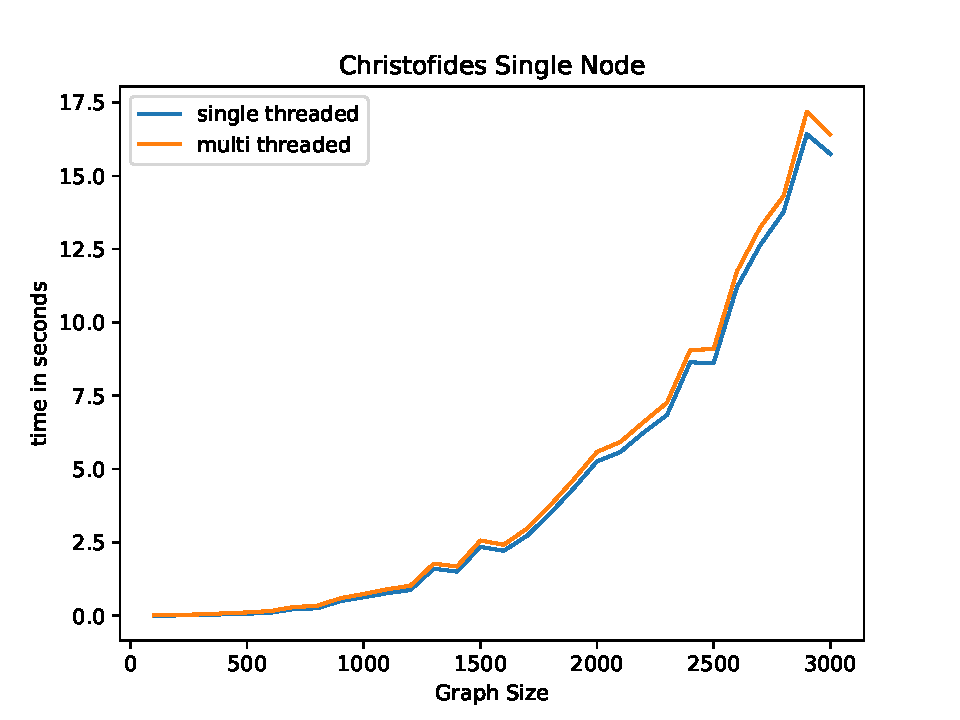
\includegraphics[width=\linewidth,height=0.8\textheight,keepaspectratio]{christofides-stmt.pdf}
  \end{figure}
  \vfill
\end{frame}

\begin{frame}[t]{Christofides Algorithm: Benchmarking}
  \vfill
  Christofides algorithm does slightly benefit w.r.t. solution weight:
  
  \begin{figure}
    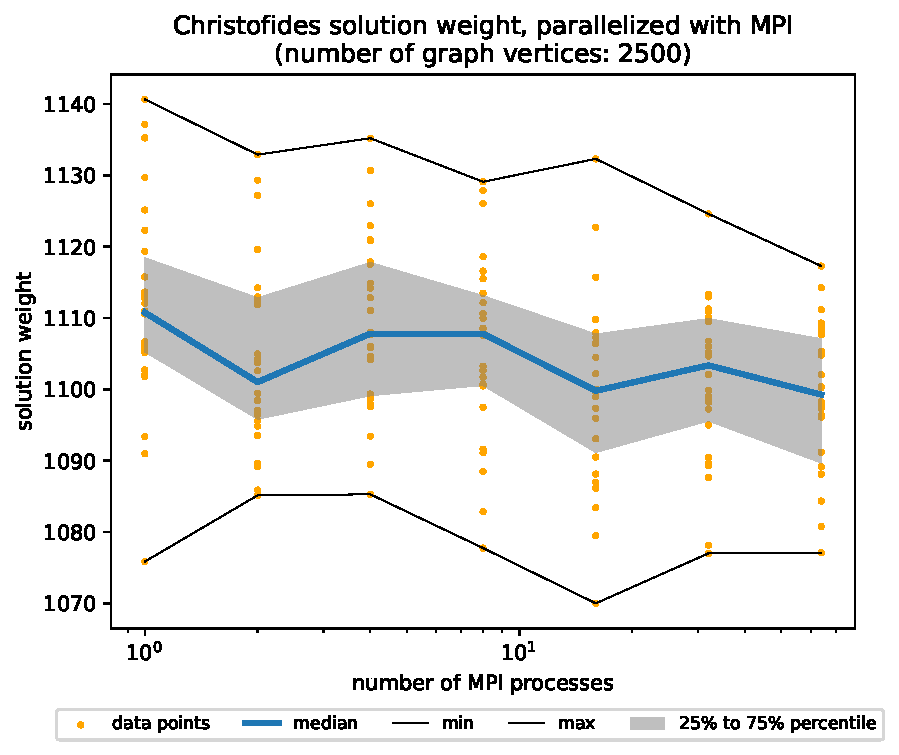
\includegraphics[width=\linewidth,height=0.8\textheight,keepaspectratio]{christofides-mpi.pdf}
  \end{figure}
  \vfill
\end{frame}
